The following diagram represents a sundial, for which the triangle, called a gnomon, casts a shadow onto the surrounding surface, which has markings and numbers representing important information. It is known that this sundial is located either between the Tropic of Cancer and the Arctic Circle or between the Tropic of Capricorn and the Antarctic Circle.

\begin{figure}[H]
    \centering
    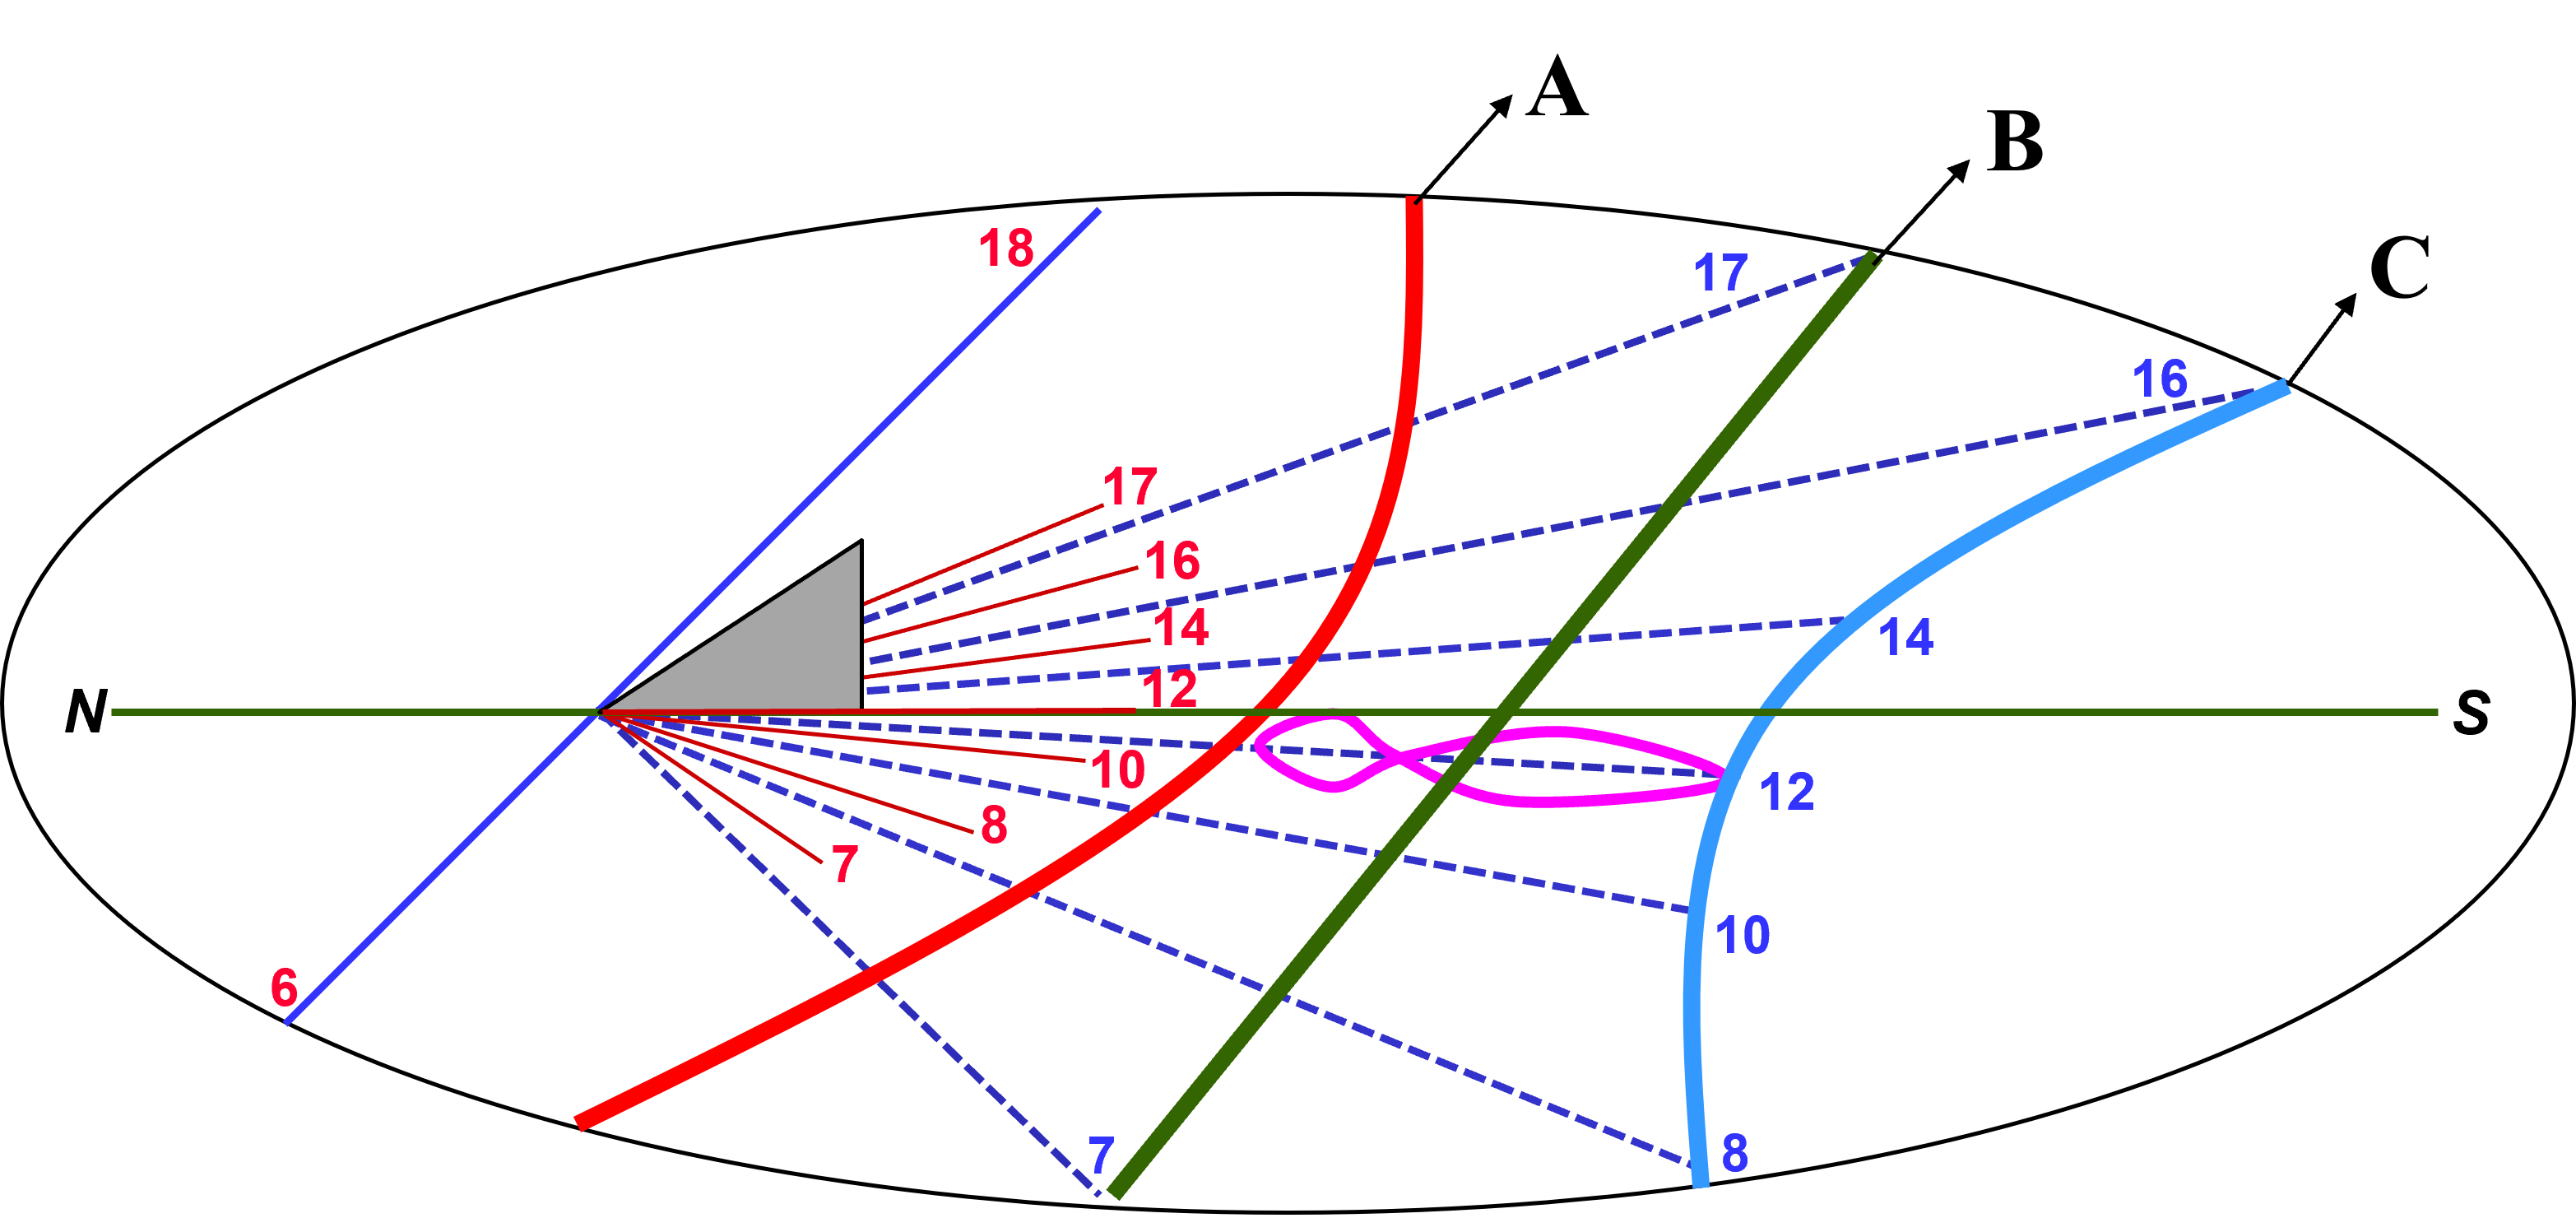
\includegraphics[width=1.0\textwidth]{2024/Theory/Figures/2024_TH_Q1_F1.png}
\end{figure}

In the image above, the angle between the dashed and solid lines for any given time is always equal to the longitude difference between the time shown by the sundial and the civil time (the time shown on your watch). For instance, the dashed line corresponding to 7h and the solid line corresponding to 7h form an angle equal to the longitude difference between the location of this sundial and the central meridian of the time zone.

Throughout the year, the shadow of the tip of the gnomon is always between curves A and C.

Read the following statements and indicate whether they are true or false. For each item, write a \textbf{T} on the answer sheet if you think the statement is true and an \textbf{F} if you think the statement is false. \textbf{There is no need to explain your answers.}

\begin{enumerate}[label=(\alph*)]
    \item This sundial will only function properly if it is located in the southern hemisphere.

    \item Curve \textbf{A} represents the trajectory of the shadow of the tip of the gnomon throughout the winter solstice (in the hemisphere the sundial is located in).

    \item Line \textbf{B} represents the trajectory of the tip of the gnomon's shadow throughout the equinoxes.

    \item The solid radial lines provide the mean local solar time.

    \item  The analemma shape around the dashed line corresponding to 12h shows the position of the tip of the gnomon's shadow during the true solar noon at the central meridian of the time zone throughout the year.
\end{enumerate}